%!TEX root = TQFTnotes.tex
%%%%%%%%%%%%%%%
\chapter{Duality in 2-categories}\label{c:duality-2cat}

Recall that for an object $X$ in a monoidal category, we have defined the
notion of left and right duals. We will now extend this notion to objects and
1-morphisms in a weak 2-category $\calC$. Doing it for objects requires
defining a monoidal structure on $\calC$; duality for 1-morphisms (also known as
adjunction) can be defined in any 2-category.

Throughout this section $\calC$ is a weak 2-category.
%%%%%%%%%%%%%%%%%%%%%%%%%%%%%%%%
\section{Adjunction for 1-morphisms}\label{s:adjunction}
\begin{definition}\label{d:adjunction}\index{adjunction!in 2-category}
  Let $\calC$ be a weak 2-category. An \emph{adjunction} in $\calC$ is the
  following data:
  \begin{itemize}
    \item A pair of 1-morphisms $f\in\Hom(X,Y)$, $g\in \Hom(Y,X)$
    \item A 2-morphism $\eta\colon 1_X\to g\circ f$ (unit of adjunction)
    \item A 2-morphism $\eps\colon f\circ g\to 1_Y$ (counit of adjunction)
  \end{itemize}
  satisfying the adjunction equations:
  \begin{equation}\label{e:adjunction}
    \begin{aligned}
      &(f\xto{} f \circ 1_X \xto{1_f\circ \eta}
        f\circ g\circ f \xto{\eps \circ 1}
        f\circ 1_Y \xto{} f)=1_f\\
      &(g\xto{}  1_X \circ g \xto{\eta\circ 1_g}
        g\circ f\circ g \xto{1 \circ \eps}
        1_X\circ g \xto{} g)=1_g
    \end{aligned}
  \end{equation}

  In this situation, we say that $f$ is the \emph{left
  adjoint}\index{adjoint!left} of $g$ and $g$ is the \emph{right
  adjoint}\index{adjoint!right} of $f$; we will write $$
  X\xrightleftharpoons[g]{f}Y. $$ Alternative notation for adjunction is
  $f\dashv g$; in both notations, the unit and the counit 2-morphisms are
  implicit.
\end{definition}

To understand the adjunction equations, we can use pasting diagrams to describe
the 2-morphisms in the left-hand side of these equations:

\begin{tikzpicture}
    \node (x1) at (0,0) {$X$};
    \node (y1) at (1.2,0) {$Y$};
    \node (x2) at (2.4,0) {$X$};
    \node (y2) at (3.6,0) {$Y$};
    \draw[->] (x1)--(y1) node[pos=0.5,scale =0.7,above]{$f$};
    \draw[->] (y1)--(x2) node[pos=0.5,scale =0.7,above]{$g$};
    \draw[->] (x2)--(y2) node[pos=0.5,scale =0.7,above]{$f$};
    \draw[->] (x1) to[bend left=50] node[pos=0.8,scale =0.7,above]{$1_X$} (x2);
    \draw[->] (x1) to [bend left=55] node[scale =0.7,above]{$f$} (y2);
    \draw[2morphism, ->] (1.2, 0.6)--(1.2,0.2) node[pos = 0.5,scale
    =0.7,right]{$\eta$};
    \draw[->] (y1) to[bend right=50] node[pos=0.2,scale =0.7,below]{$1_Y$}
    (y2);
    \draw[->] (x1) to [bend right=55] node[scale =0.7,below]{$f$} (y2);
    \draw[2morphism, ->] (2.4, -0.2)--(2.4,-0.6) node[pos = 0.5,scale
    =0.7,right]{$\eps$};
\end{tikzpicture}
\qquad
\begin{tikzpicture}
    \node (y1) at (0,0) {$Y$};
    \node (x1) at (1.2,0) {$X$};
    \node (y2) at (2.4,0) {$Y$};
    \node (x2) at (3.6,0) {$X$};
    \draw[->] (y1)--(x1) node[pos=0.5,scale =0.7,above]{$g$};
    \draw[->] (x1)--(y2) node[pos=0.5,scale =0.7,above]{$f$};
    \draw[->] (y2)--(x2) node[pos=0.5,scale =0.7,above]{$g$};
    \draw[->] (x1) to[bend left=50] node[pos=0.2,scale =0.7,above]{$1_X$} (x2);
    \draw[->] (y1) to [bend left=55] node[scale =0.7,above]{$g$} (x2);
    \draw[2morphism, ->] (2.4, 0.6)--(2.4,0.2) node[pos = 0.5,scale
    =0.7,right]{$\eta$};
    \draw[->] (y1) to[bend right=50] node[pos=0.7,scale =0.7,below]{$1_Y$}
    (y2);
    \draw[->] (y1) to [bend right=55] node[scale =0.7,below]{$g$} (x2);
    \draw[2morphism, ->] (1.2, -0.2)--(1.2,-0.6) node[pos = 0.5,scale
    =0.7,right]{$\eps$};
\end{tikzpicture}


Alternatively --- and more intuitively --- we can use string diagrams.
Namely, we will illustrate 2-morphisms $\eta$ and $\eps$ by string diagrams as
in \firef{f:adjunction_units}. Then the adjunction equations become the
equations of \firef{f:AdjunctionStringDiagram}, justifying our choice of
graphical depiction.
\begin{figure}[ht]
  \begin{center}
    \begin{tikzpicture}[thick]
      \begin{scope}
        \node at (-.5, .5) {$\eta =$};
        %%
        \coordinate (LT) at (0, 1);
        \coordinate (LB) at (0, 0);
        \coordinate (RT) at (2, 1);
        \coordinate (RB) at (2, 0);
        \node (f) [label=below:$f$] at (.5, 0) {};
        \node (g) [label=below:$g$]  at (1.5, 0) {};
        \path[spath/save = arc] (f) arc (180: 0: 0.5 cm);
        %% fills
        \fill [lightblue] [spath/use=arc] -- (RB)--(RT)--(LT)--(LB)--cycle;
        \fill [lightred] [spath/use=arc]--cycle;
        %%
        \draw[spath/use=arc];
        \node[below right] at (LT) {$X$};
        \node[above] at (1,0) {$Y$};
      \end{scope}

      \begin{scope}[xshift = 5cm]
        \node at (-.5, .5) {$\eps =$};
        %%%%%%%%%
        \coordinate (LT) at (0, 1);
        \coordinate (LB) at (0, 0);
        \coordinate (RT) at (2, 1);
        \coordinate (RB) at (2, 0);
        \node (g) [label=above:$g$] at (.5, 1) {};
        \node (f) [label=above:$f$]  at (1.5, 1) {};
        \path[spath/save = arc] (g) arc (180: 360: 0.5 cm);
        %% fills
        \fill [lightred] [spath/use=arc] -- (RT)--(RB)--(LB)--(LT)--cycle;
        \fill [lightblue] [spath/use=arc]--cycle;
        %%
        \draw[spath/use=arc];
        \node[above right] at (LB) {$Y$};
        \node[below] at (1,1) {$X$};
      \end{scope}
    \end{tikzpicture}
    \caption{String diagrams for adjunction unit and counit.}
    \label{f:adjunction_units}
  \end{center}
\end{figure}

\begin{figure}[ht]
  \begin{center}
    \begin{tikzpicture}[thick]
      \begin{scope}
        \coordinate (LT) at (0,2);
        \coordinate (LB) at (0,0);
        \coordinate (RT) at (3, 2);
        \coordinate (RB) at (3, 0);
        \node[label=below:$f$] (f1) at (.9, 0){};
        \node[label=above:$f$] (f2) at (2.1, 2){};

        %%%%
        \path[spath/save=zigzag] (f1.center) -- ++(0,1) arc (180:0: 0.3 cm) arc
        (180: 360: 0.3 cm) -- (f2.center);
        %%% fills
        \fill [lightblue] [spath/use= zigzag] -- (LT) -- (LB)--(f1.center);
        \fill [lightred] [spath/use= zigzag] -- (RT) -- (RB) -- (f1.center);
        %%% draw line
        \draw[spath/use= zigzag];
        \node[right] at (0, 1) {$X$};
        \node[left] at (3, 1) {$Y$};
        %%%
        \node at (3.5, 1) {=};
        \fill [lightblue] (4, 2) rectangle (5, 0);
        \fill [lightred] (5, 2) rectangle (6, 0);
        \draw (5, 2) -- (5, 0);
        \node[right] at (4, 1) {$X$};
        \node[left] at (6, 1) {$Y$};
        \node[above] at (5,2) {$f$};
        \node[below] at (5,0) {$f$};
      \end{scope}

      \begin{scope}[yshift = -4cm]
        \coordinate (LT) at (0,2);
        \coordinate (LB) at (0,0);
        \coordinate (RT) at (3, 2);
        \coordinate (RB) at (3, 0);
        \coordinate (g1) at (.9, 2);\node[above] at (g1) {$g$};
        \coordinate (g2) at (2.1, 0);\node[below] at (g2) {$g$};

        \path[spath/save=zigzag] (g1) -- ++(0,-1) arc (180:360: 0.3 cm) arc
        (180: 0: 0.3 cm) -- (g2);
        %%% fills
        \fill [lightred] (LT)  [spath/use= zigzag] -- (LB) -- (LT);
        \fill [lightblue] [spath/use= zigzag] -- (RB) -- (RT) -- (g1);
        %%% draw line
        \draw[spath/use= zigzag];
        \node[right] at (0, 1) {$Y$};
        \node[left] at (3, 1) {$X$};
        %%%%%%%%%
        \node at (3.5, 1) {=};
        %%%%%%%%
        \fill [lightred] (4, 2) rectangle (5, 0);
        \fill [lightblue] (5, 2) rectangle (6, 0);
        \node[right] at (4, 1) {$Y$};
        \node[left] at (6, 1) {$X$};
        \draw (5, 2) -- (5, 0);

      \end{scope}

    \end{tikzpicture}
    \caption{Adjunction equations via string diagrams}
    \label{f:AdjunctionStringDiagram}
  \end{center}
\end{figure}

The definition of adjunction given above generalizes two well-known examples:
duality in a monoidal category and adjunction of functors.

\begin{example}\label{x:adjunction-monoidal}
  Let $\calC$ be a monoidal category, and let $B\calC$ be the corresponding
  2-category with one object as defined in \exref{x:BC}. Then the definition of
  adjunction for 1-morphisms in $B\calC$ coincides with the notion of dual pairs
  of objects in $\calC$: $A\dashv B$ as 1-morphisms in $B\calC$ if and only if
  $B$ is the right dual of $A$ in $\calC$.
\end{example}

\begin{theorem}\label{t:adjunction-cat}\index{adjunction!for functors}
  Let $\cat$ be the 2-category of small categories. Let $f\colon \calC\to
  \calD$, $g\colon \calD\to \calC$ be 1-morphisms in $\cat$ \textup{(}i.e., functors
  between the corresponding categories\textup{)}. Then defining adjunction data
  $\eta, \eps$ as in \deref{d:adjunction} is equivalent to defining
  a functorial isomorphism
  \begin{equation}\label{e:adjunction-cat}
    \Hom_{\calD}(f(-), -)\simeq \Hom_{\calC}(-, g(-)).
  \end{equation}
\end{theorem}
\begin{proof}
  (Sketch of proof)

  Suppose we are given a functorial isomorphism \eqref{e:adjunction-cat}. Then
  for any object $c\in \calC$, we have isomorphism $\Hom_{\calD}(f(c),
  f(c))\simeq \Hom_{\calC}(c, g(f(c)))$. In particular, applying it to the
  identity morphism $1_{f(c)}$, we get a canonical element $\eta\in \Hom(c,
  g(f(c)))$, or equivalently, a functorial morphism $\id_{\calC}\to g\circ f$,
  which can be used as the unit of adjunction as in \deref{d:adjunction}.
  Similarly we get a functorial morphism $\eps\colon fg(d)\to d$, which is the
  counit of adjunction. The adjunction relations shown in
  \firef{f:AdjunctionStringDiagram} follow from the functoriality of
  \eqref{e:adjunction-cat}.

  We leave the construction in the opposite direction as an exercise to the
  reader.

\end{proof}

Adjoint functors between categories frequently appear as
``restriction--induction'' pairs; we give several examples below.
\begin{example}\label{x:coset-bimodule}
  Let $G$ be a finite group and $H\subset G$ a subgroup. Consider the
  restriction functor $\Res\colon \Rep G\to \Rep H$. Then it has a left adjoint
  called the induction functor $\Ind \colon \Rep H\to \Rep G$. The adjunction
  relation
  $$
  \Hom_G(\Ind V, W)\simeq \Hom_H(V, \Res W), \qquad V\in \Rep H, W\in \Rep G
  $$
  is known as \emph{Frobenius reciprocity}\index{Frobenius reciprocity};
  from our point of view, it is the
  definition of the induction functor.
 \end{example}

\begin{example}\label{x:abelian-groups-duality}
  Let $\calC$ be the category of abelian groups. It has an obvious forgetful
  functor $F\colon \calC\to\sets$. This functor has a left adjoint
  $I\colon\sets\to \calC$; namely, $I(S)$ is the abelian group freely generated
  by elements of $S$. Again, we take it as the definition of ``freely
  generated''; the nontrivial fact is that such a left adjoint exists.
\end{example}


Returning to adjunction in an arbitrary 2-category $\calC$,
here are some useful results about adjunctions.

\begin{lemma}\label{l:adjunction-unique}
  Let $f\colon X\to Y$ be a 1-morphism in a weak 2-category $\calC$. Then
  the remaining adjunction data, $g, \eta, \eps$ \textup{(}as in
  \deref{d:adjunction}\textup{)}, if it exists, is unique up to unique isomorphism: if
  $(f,g,\eta,\eps)$ and $(f, \tilde g, \tilde \eta, \tilde \eps)$ are two
  different sets of adjunction data with the same $f$, then there is a
  unique 2-morphism $\al\colon g\to \tilde g$ which makes the appropriate
  diagrams commutative.
\end{lemma}
We leave the proof as an exercise (see also \cite[Section IV.1]{mac-lane}).

A variation of this is the following result.
\begin{lemma}\label{l:adjunction-unique2}
  The unit of the adjunction is uniquely determined by the remaining
  adjunction data: if $(f, g, \eta, \eps)$ and $(f, g, \eta', \eps)$ are two
  sets of adjunction data, then
  $\eta=\eta'$.

  Similarly, the counit $\eps$ of adjunction is uniquely determined by
  $(f,g, \eta)$.

  Moreover, if $(f, g, \eta, \eps)$ satisfies one of the adjunction equations
  \eqref{e:adjunction}, and $(f, g, \eta', \eps)$ satisfies the other one,
  then $\eta=\eta'$ \textup{(}and thus satisfies both equations\textup{)}.
\end{lemma}
\leref{l:adjunction-unique} and \leref{l:adjunction-unique2} are analogs of
\thref{t:dual_unique1} and \ecref{ec:coev-unique} for monoidal categories,
and the proofs are similar (see \cite[Lemma 2.3.8]{lurie-cobordism}).



The notion of adjunction is closely related to the notion of equivalence. Recall
that a 1-morphism $f\colon X\to Y$ in a 2-category is called an
\emph{equivalence}\index{equivalence!of 1-morphisms} if there exists $g\colon
Y\to X$ such that $fg\simeq 1_Y$, $gf\simeq 1_X$. (This is a weaker version of
an invertible morphism --- requiring that $fg=1_Y$ would be too strict, since
1-morphisms in a 2-category are usually only isomorphic, not equal.)

\begin{lemma}\label{l:adjoint-equivalence}
  If $f\colon X\to Y$, $g\colon Y\to X$ are 1-morphisms in a weak
  2-category such that $fg\simeq 1_Y$, $gf\simeq 1_X$, then
  $g$ is both a left and a right adjoint of $f$.
\end{lemma}
\begin{proof}
  Choose arbitrary isomorphisms $\al\colon fg\isoto 1_Y$, $\be \colon gf\isoto
  1_X$. Then the composition
  $$
  \theta = (f\xto{ \al^{-1} \ccirc 1_f} fgf\xto{1_f\ccirc \be} f)
  $$
  is an invertible 2-morphism $f\to f$. Thus, setting $\eta = (\theta^{-1}\ccirc
  1_g) \al^{-1}$, $\eps = \be$ we see that the so-defined $\eta, \eps$ satisfy one
  of the adjunction equations. In a similar way we can find $\eta', \eps$ which
  satisfy the other adjunction equation. Now the result follows from
  \leref{l:adjunction-unique2}.
\end{proof}
In other words, every equivalence can be upgraded to an adjoint equivalence.



%In a monoidal category, given an object $B$ which has a left dual $B^*$,
%we have functorial isomiorphisms
%$$
%\Hom (A\otimes B, C)\simeq \Hom(A, C\otimes B^*)
%$$
%given by the picture below.
%
%A similar statement holds in a weak 2-category: we have a bijection
%$$
%\Hom(f \circ g,h )\simeq \Hom(f, h\circ g^*)
%$$
%where $g^*$ is right adjoint of $g$.
%
%FIXME

%%%%%%%%%%%%%%%%%%%%%%%%%%%%%%%%%%%%%%%%%%%%%%%%%%%%%%%%%%%%%%%%%%%%%%%%
\section{Dual objects in 2-categories}\label{s:coherent-dual-pair}

Let us now talk about dual objects in $\calC$. It only makes sense
if $\calC$ has a monoidal structure; thus, in this section we assume that
$\calC$ is a monoidal weak 2-category.

Recall that in a (usual) monoidal category, we defined a dual pair as the data
$(A,B, \ev, \coev)$, where $\ev\colon A\otimes B\to \one$,
$\coev \colon \one \to B\otimes A$ are morphisms satisfying the zigzag (or
rigidity) relations $z_A= 1_A$, $z_B = 1_B$, where
\begin{equation}\label{e:zigzags}
    \begin{aligned}
        z_A&= (A\xto{1_A\otimes \coev} A\otimes B \otimes A \xto{\ev\otimes
        1_A} A)\\
        z_B &= (B \xto{\coev \otimes 1_B} B\otimes A \otimes B
        \xto{1_B\otimes\ev} B)
\end{aligned}
\end{equation}
(see \deref{d:dual-object}).

We now want to upgrade this definition, defining the notion of a dual pair in a
monoidal weak 2-category. In this case, it makes no sense to require $z_A=1_A$,
$z_B=1_B$; instead, we need isomorphisms $\al \colon z_A\to 1_A$, $\be\colon
z_B\to 1_B$. Moreover, it is natural to expect that these isomorphisms
themselves should satisfy some compatibility relations. Following
\cite{pstragowski}, we will impose the following relations.

Let $zz_+$ be the ``double zigzag'' 1-morphism
\begin{equation}
  \begin{aligned}
    zz_+&= (A\otimes B \xto{1_A\otimes \coev\otimes 1_B}
            A \otimes (B \otimes A) \otimes B \xto {\ev \otimes \ev}
            \one )\\
    & \qquad
    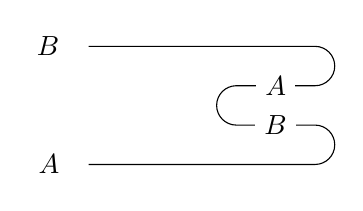
\begin{tikzpicture}
      \node[label = left:$B$] (B) at (0,0){};
      \node[label = left:$A$] (A) at (0,-1.5){};
      \draw (B)-- +(3,0)  arc (90:-90:0.25)
                                 -- +(-1,0) arc (90:270:0.25)
                                 -- +(1,0) arc(90:-90:0.25)
                                 -- (A);
      \node[fill = white] at (2.5,-0.5) {$A$};
      \node[fill = white] at (2.5,-1) {$B$};
    \end{tikzpicture}
  \end{aligned}
\end{equation}
(we have turned the picture 90 degrees counterclockwise, to match our
convention that in 2-categories, 1-morphisms go ``from left to right'').

Then we have two different 2-morphisms $zz_+\to \ev$: $\al\otimes 1$, obtained
by using $\al$ on the lower part of zigzag, and $1\otimes \be$, obtained by using
$\be$ on the top part of zigzag (we leave it to the reader to write them
algebraically).

It is natural to require that these 2-morphisms are equal:
\begin{equation}\label{e:swallowtail1}
  \begin{tikzpicture}[vcenter]
    \begin{scope}
      % objects
      \node (x) at (0,0) {$A\otimes B$};
      \node (y) at (3,0) {$\one$};
      % 1-morphisms
      \draw[->, thick, bend left=35] (x) to node[above] {$zz_+$} (y);
      \draw[->, thick, bend right=35] (x) to node[below] {$\ev$} (y);
      % 2-morphism as a double arrow between the 1-morphisms
      \draw[2morphism,->] (1.5,0.3) -- (1.5,-0.3)
            node[midway, right, scale=0.8] {$\al\otimes 1$};
    \end{scope}
    \node at (3.8,0) {$=$};
    \begin{scope}[xshift=5cm]
      % objects
      \node (x) at (0,0) {$A\otimes B$};
      \node (y) at (3,0) {$\one$};
      % 1-morphisms
      \draw[->, thick, bend left=35] (x) to node[above] {$zz_+$} (y);
      \draw[->, thick, bend right=35] (x) to node[below] {$\ev$} (y);
      % 2-morphism as a double arrow between the 1-morphisms
      \draw[2morphism,->] (1.5,0.3) -- (1.5,-0.3)
      node[midway, right, scale=0.8] {$1\otimes \be$};
    \end{scope}
  \end{tikzpicture}
\end{equation}
Similarly, we can define a 1-morphism $zz_-\colon \one\to B\otimes A$ by the
picture below
$$
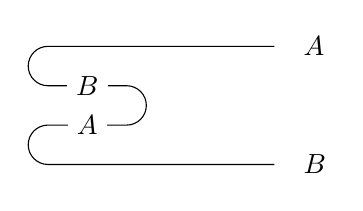
\begin{tikzpicture}
  \node[label = right:$A$] (A) at (0,0){};
  \node[label = right:$B$] (B) at (0,-1.5){};
  \draw (A)-- +(-3,0)  arc (90:270:0.25)
  -- +(1,0) arc (90:-90:0.25)
  -- +(-1,0) arc(90:270:0.25)
  -- (B);
  \node[fill = white] at (-2.5,-0.5) {$B$};
  \node[fill = white] at (-2.5,-1) {$A$};
\end{tikzpicture}
$$
As with $zz_+$, there are two different 2-morphisms $zz_-\to \coev$, and we
require that they
are equal:
\begin{equation}\label{e:swallowtail2}
  \begin{tikzpicture}[vcenter]
    \begin{scope}
      % objects
      \node (x) at (0,0) {$\one$};
      \node (y) at (3,0) {$B\otimes A$};
      % 1-morphisms
      \draw[->, thick, bend left=35] (x) to node[above] {$zz_-$} (y);
      \draw[->, thick, bend right=35] (x) to node[below] {$\coev$} (y);
      % 2-morphism as a double arrow between the 1-morphisms
      \draw[2morphism,->] (1.5,0.3) -- (1.5,-0.3)
      node[midway, right, scale=0.8] {$1\otimes \al$};
    \end{scope}
    \node at (4,0) {$=$};
    \begin{scope}[xshift=4.7cm]
      % objects
      \node (x) at (0,0) {$\one$};
      \node (y) at (3,0) {$B\otimes A$};
      % 1-morphisms
      \draw[->, thick, bend left=35] (x) to node[above] {$zz_-$} (y);
      \draw[->, thick, bend right=35] (x) to node[below] {$\coev$} (y);
      % 2-morphism as a double arrow between the 1-morphisms
      \draw[2morphism,->] (1.5,0.3) -- (1.5,-0.3)
      node[midway, right, scale=0.8] {$\be\otimes 1$};
    \end{scope}
  \end{tikzpicture}
\end{equation}
We will call relations \eqref{e:swallowtail1}, \eqref{e:swallowtail2}
\emph{swallowtail relations}\index{swallowtail relations}.
The name comes from their geometric interpretation
in terms of 2-cobordisms, which we will discuss in the next section.

Thus, we are led to the following definition (we use the terminology of
\cite{pstragowski}).

\begin{definition}\label{d:coherent-dual-pair}\index{dual pair!in 2-category}
  A \emph{coherent dual pair} in a weak monoidal 2-category
  $\calC$ is the following collection of
  data:
  \begin{itemize}
    \item Objects $A, B\in \calC$.
    \item 1-morphisms $\ev  \colon A\otimes B\to \one$,
      $\coev \colon \one \to B\otimes A$.
    \item Invertible 2-morphisms $\al \colon z_A\to 1_{A}$,
      $\be \colon z_B\to 1_{B}$, where $z_A$, $z_B$ are defined
      by \eqref{e:zigzags}.
  \end{itemize}
  such that $\al, \be$ satisfy the swallowtail relations
  \eqref{e:swallowtail1}, \eqref{e:swallowtail2}.

  In this case, we say that $B$ is a right dual of $A$, and $A$ is a left
  dual of $B$.
\end{definition}


\begin{lemma}\label{l:dual-pair-upgrade}
  Let $(A, B, \ev, \coev, \al, \be)$ be as in the definition of
  coherent dual pair, but without the swallowtail relations.
  Then one can replace $\be$ by another
  2-isomorphism $\tilde \be$ so that
  $(A, B, \ev, \coev, \al, \tilde \be)$ is a coherent dual pair.
\end{lemma}

In other words, if you have any isomorphisms $z_A\to 1_A$, $z_B\to 1_B$,
then you can modify one of them to satisfy the swallowtail relations.

The proof of this lemma is similar to \leref{l:adjoint-equivalence}, where
we also argued that given a pair of isomorphisms, we can modify one of them
to satisfy an additional consistency requirement (in that case, the adjunction
property). We refer the reader to \cite[Theorem 2.7]{pstragowski} for
details of the proof.

Recall that for a weak 2-category $\calC$, we defined a (usual) category
$h\calC$ by making 1-morphisms that were isomorphic in $\calC$ equal in
$h\calC$, see \deref{d:hC}. Then \leref{l:dual-pair-upgrade} implies that
any dual pair $(A,B, \ev, \coev)$ in $h\calC$ can be ``upgraded'' to a
coherent dual pair in $\calC$. In particular, this implies the following.

\begin{corollary}\label{c:dual-objects-2cat}
  An object $A\in \calC$ has a right \textup{(}respectively, left\textup{)} dual in $\calC$
  if and only if it has the right \textup{(}respectively, left\textup{)}
  dual in the homotopy category $h\calC$.
\end{corollary}

We can also ask whether, for a given $A$, all coherent dual pairs
including it are equivalent. To do that, we define the notion of
an isomorphism of dual pairs, which consists of a pair of isomorphisms of
objects and 2-isomorphisms between evaluation and coevaluation; details
can be found in \cite[Section 2.2]{pstragowski}.


\begin{theorem}\label{t:coh-dual-pair-unique}
    Let $A$ be an object in $\calC$, and let $(A,B, \dots)$,
    $(A, B', \dots)$ be two coherent dual pairs including $A$.
    Then there exists an isomorphism between them which is identity on $A$.
\end{theorem}

(This is a simplified version; a more accurate statement, which also
answers the question of whether such an isomorphism is unique, is given
in \cite[Theorem 2.14]{pstragowski} and says that the 2-groupoid of
coherent dual pairs is equivalent to the 2-groupoid of
objects in $\calC$ which have a right dual.)

In summary, we see that any dual pair in $h\calC$ can be ``upgraded'' to a
coherent dual pair in $\calC$, and any two such upgrades are isomorphic. Thus,
producing such a coherent dual pair is essentially equivalent to producing an
object $A\in \calC$ which has a right dual in $h\calC$.


\begin{remark}
  In all our discussions in this section, we ignored associativity and unit
  isomorphisms in the monoidal 2-category $\calC$. Technically speaking,
  this is not correct, and we must include them. Unfortunately, if we do
  that, all diagrams become hopelessly complicated --- for example, here is
  the diagram of one of the swallowtail relations in all glorious detail, taken
  from \cite{pstragowski}:

  
\includegraphics[width = 0.8\textwidth]{swallowtail.pdf}
\end{remark}


Finally, we give the following definitions.

\begin{definition}\label{d:category-duals}\index{category!with duals}
  A symmetric monoidal weak 2-category $\calC$ is called a \emph{category with
  duals} if
  \begin{enumerate}
    \item Every object $A\in \calC$ is rigid, i.e., has a dual in $\calC$.
    \item Every 1-morphism has both left and right adjoints.
  \end{enumerate}
\end{definition}

\begin{definition}\label{d:fully-dualizable-2cat}\index{fully dualizable object}
  An object $A$ in a symmetric monoidal weak 2-category $\calC$ is called
  \emph{fully dualizable} if it lies in some subcategory $\calD\subset
  \calC$ which is a category with duals.
\end{definition}

It is not difficult to show (see \cite[Proposition
  4.2.3]{lurie-cobordism}) that an object $A$ is fully dualizable if and only if $A$ has a
dual $A^*$ and the corresponding evaluation and coevaluation 1-morphisms
have left and right adjoints. Moreover, the existence of adjoints for $\ev$
implies the existence of adjoints for $\coev$ and vice versa.

%%%%%%%%%%%%%%%%%%%%%%%%%%%%%%%
\section{Serre functor}\label{s:serre}
Let $\calC$ be a symmetric monoidal 2-category, and let $A$ be a fully
dualizable object in $\calC$. Denote by $B=A^*$ the dual of $A$ and by
$\ev\colon A\otimes B\to \one$, $\coev\colon \one \to B\otimes A$ the
corresponding evaluation and coevaluation morphisms.

By the definition of a fully dualizable object, the morphism $\ev$ must have right and
left adjoints, which we will denote by $\ev^R$, $\ev^L$ respectively. Both of
them are morphisms $\one \to A\otimes B$; thus, we have adjunctions
\begin{align*}
&A\otimes B \xrightleftharpoons[\ev^R]{\ev}\one,\\
&\one \xrightleftharpoons[\ev]{\ev^L}A \otimes B.
\end{align*}

It is natural to ask what is the relation between these adjoints and the
coevaluation morphism $\coev\colon \one \to B \otimes A$. Note that here $A$ and
$B$ go in the opposite order, but since $\calC$ is a symmetric monoidal
category, we can use the commutativity isomorphism to exchange them, defining
$\widetilde\coev = c_{B,A}\coev\colon \one \to A\otimes B$. It turns out that
while in general, $\widetilde\coev$ is different from $\ev^L$, $\ev^R$, they can
be related using the so-called \emph{Serre automorphism}.

\begin{definition}\label{d:serre}\index{Serre automorphism}
  Let $A$ be a fully dualizable object in $\calC$. The Serre morphism $S_A$ is the
  1-morphism $A\to A$ defined by
  \begin{equation}\label{e:serre-formula}
    S_A=\Bigl(
     A\xto{1_A\otimes \ev^R} A\otimes A\otimes B \xto{c_{A,A}\otimes 1_B}
     A\otimes A\otimes B \xto{1_A\otimes \ev} A
         \Bigr).
   \end{equation}
   Graphically, this composition is represented by the picture
   \eqref{e:serre-picture} below:
   \begin{equation}\label{e:serre-picture}
     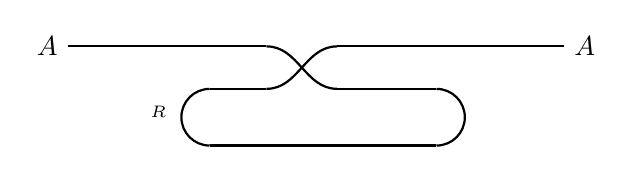
\begin{tikzpicture}[thick, baseline=0, scale=0.9]
       %% Input A on the left
       \node[left] at (0,1) {$A$};
       %% Output A on the right
       \node[right] at (7,1) {$A$};

       %% Input A goes from left to the braiding at x=2.8
       \draw (0,1) -- (2.8,1);

       %% ev^R cap (creates A and B): opens at x=1.7, with endpoints at
       %% (2, 0.4) (= new A, top) and (2, -0.4) (= new B, bottom)
       \draw (2, 0.4) arc (90:270:0.4);
       \node[left] at (1.55,0) {\small$\ev^R$};

       %% new A continues from (2, 0.4) to braiding at x=2.8
       \draw (2, 0.4) -- (2.8, 0.4);

       %% new B continues from (2,-0.4) to ev at x=5.2
       \draw (2, -0.4) -- (5.2, -0.4);

       %% Braiding c_{A,A}: input A (y=1) crosses with new A (y=0.4)
       \draw (2.8, 1) to[out=0, in=180] (3.8, 0.4);  % input A goes down
       \draw (2.8, 0.4) to[out=0, in=180] (3.8, 1);  % new A goes up

       %% After braiding: new A at y=1 (continues to output),
       %% input A at y=0.4 (continues to ev)
       \draw (3.8, 1) -- (7, 1);
       \draw (3.8, 0.4) -- (5.2, 0.4);

       %% ev cup (closes input A with new B): opens at x=5.6
       \draw (5.2, 0.4) arc (90:-90:0.4);
       \node[right] at (5.65,0) {\small$\ev$};
     \end{tikzpicture}
   \end{equation}
   where the input/output of $S_A$ are the two horizontal strands labeled $A$,
   and the loop formed by $\ev^R$ and $\ev$ represents the auxiliary
   $A\otimes B$ pair created and then annihilated; the crossing in the middle
   is the symmetry isomorphism $c_{A,A}$.
\end{definition}

\begin{remark}
  The name ``Serre automorphism'' is motivated by the relation of this to Serre
  duality in the category of coherent sheaves on projective varieties; see
  \cite[Remark 4.2.4]{lurie-cobordism}.
\end{remark}


\begin{theorem}\label{t:serre}
  Let $A$ be a fully dualizable object in $\calC$ and let
  $S_A\colon A\to A$ be the Serre morphism defined by \deref{d:serre}.
   Then $S_A$ is invertible, and we have an isomorphism of 1-morphisms
   \begin{align*}
   \ev^L&\simeq (S\otimes 1_B)  \widetilde \coev \\
   \ev^R&\simeq (S^{-1}\otimes 1_B)\widetilde \coev.
   \end{align*}
\end{theorem}
We refer the reader to \cite[Section 3.1]{pstragowski} for the proof.

In particular, this theorem implies that if the Serre automorphism is trivial
(i.e., one has a 2-isomorphism $S_A\simeq 1_A$), then $\ev, \widetilde\coev$ are
two-sided adjoints of each other. More precisely, a choice of an isomorphism
$S_A\simeq 1_A$ defines the unit and counit of adjunctions $\ev\dashv
\widetilde\coev$, $\widetilde\coev\dashv\ev$.



%%%%%%%%%%%%%%%%%%%%%%%%%%%%%%%
\section{Duality in $\Linlf$}\label{s:lin-duals}
As the simplest example of duality in a 2-category, let us consider the
2-category $\Linlf$ of locally finite $\kk$-linear  categories, introduced in
\seref{s:deligne-product}. Recall that objects of that category are $\kk$-linear
abelian categories such that all $\Hom$ spaces are finite-dimensional and every
object has finite length. This 2-category has a natural symmetric monoidal
structure, given by Deligne's product $\boxtimes$.

Let us now analyze which objects of $\Linlf$ are rigid, i.e., for which
categories $\calC$ there exist a category $\calD$ and functors
\begin{align*}
  \eta&\colon \vecf \to \calD\boxtimes \calC\\
  \epsilon&\colon \calC\boxtimes \calD\to \vecf
\end{align*}
satisfying the rigidity axioms. Clearly, defining the functor $\eta$ is equivalent
to choosing an object
$$
  e=\eta (\kk)=\bigoplus_{i=1}^k Y_i\boxtimes X_i\in \calD\boxtimes \calC
$$
together with functorial isomorphisms
\begin{equation}\label{e:rigidity-lin}
  \begin{aligned}
    X&\simeq \bigoplus \eps(X,Y_i)\otimes X_i\\
    Y&\simeq \bigoplus \eps(X_i,Y)\otimes Y_i
  \end{aligned}
\end{equation}
for every $X\in \calC$, $Y\in \calD$.

\begin{theorem}\label{t:dualizable-linear}
  Let $\kk$ be an algebraically closed field of characteristic zero. Then a
  category $\calC\in \Linlf$ is rigid as an object of $\Linlf$ if and only if it
  is semisimple and has finitely many isomorphism classes of simple objects. In
  this case, the dual category $\calD$ is equivalent to the category of
  $\kk$-linear functors $\calC\to \vecf$; under this equivalence, the counit
  $\eps\colon \calC\boxtimes\calD\to \vecf$ is given by
  $$
    \eps(X,F) = F(X)\in \vecf,\qquad X\in \calC, F\in \Fun(\calC, \vecf)
  $$
  and the object $e=\bigoplus Y_i\boxtimes X_i$ is given by
  $$
    e=\bigoplus X^i \boxtimes X_i
  $$
  where the sum is over isomorphism classes of simple objects $X_i\in \calC$,
  and for such a simple object, we define
  $$
    X^i=\Hom(X_i, -)\in \Fun(\calC, \vecf).
  $$
\end{theorem}
\begin{proof}
  Our proof follows \cite[Section A.6]{bdspv}, where the proof is attributed
  to Andr\'e Henriques. (Note that they work in greater generality: they do not
  require the category to be abelian, instead imposing a weaker condition of
  Cauchy completeness.)


  First, finiteness easily follows from the observation that by
  \eqref{e:rigidity-lin}, any $X\in \calC$ is a subobject in a finite direct sum
  of copies of $X_1, \dots, X_k$. Thus, the only simple objects that can appear
  in the Jordan--H\"older series for $X$ are those simple objects that appear in
  the Jordan--H\"older series for one of the $X_i$; which implies that there are only
  finitely many of them.

  To prove semisimplicity, let $0\to A_1\to A_2\to A_3\to 0$ be a short exact
  sequence in $\calC$. Using \eqref{e:rigidity-lin}, we can rewrite it as a
  short exact sequence
  $$
  0 \to \bigoplus \eps(Y_i, A_1)\otimes X_i
    \to \bigoplus \eps(Y_i, A_2)\otimes X_i
    \to \bigoplus \eps(Y_i, A_3)\otimes X_i
  \to 0.
  $$
  Since a direct sum of complexes is exact if and only if each summand is
  exact, this implies that each complex
  $$
  K_i = \Bigl(
      0 \to  \eps(Y_i, A_1)\otimes X_i
          \to  \eps(Y_i, A_2)\otimes X_i
          \to \eps(Y_i, A_3)\otimes X_i
        \to 0
        \Bigr)
  $$
  is exact. This in turn is equivalent to the requirement that the complex of
  vector spaces
  $$
    0 \to  \eps(Y_i, A_1)
            \to  \eps(Y_i, A_2)
            \to \eps(Y_i, A_3)
    \to 0
  $$
  is exact. But each short exact sequence of vector spaces splits; thus, each
  short exact sequence $K_i$ splits, which implies that the original short
  exact sequence $0\to A_1\to A_2\to A_3\to 0$ also splits. Thus, $\calC$ is
  semisimple.

  We leave the proof of the remaining parts of the theorem as an exercise to the
  reader.
 \end{proof}

 After establishing duality for objects of $\Linlf$, we can turn to establishing
 duality for 1-morphisms. For simplicity, we give the answer for a slightly
 smaller 2-category of \emph{finite} $\kk$-linear categories.

 \begin{definition}\label{d:finite}
    A locally finite $\kk$-linear category $\calA$ is called \emph{finite}\index{category!finite} if
    it satisfies the following additional conditions
    \begin{itemize}
      \item The set of isomorphism classes of simple objects in $\calA$ is
        finite.
      \item There are enough projective objects.
    \end{itemize}
\end{definition}
A more detailed discussion of finite categories can be found, e.g., in
\cite[Section 1.8]{etingof-fusion}.

 \begin{theorem}\label{t:exact-adjoint}
  Assume that $\kk$ is an algebraically closed field of characteristic zero. Let
  $\calC$, $\calD\in \Linlf$ be finite $\kk$-linear categories. Then a functor
  $F\colon \calC\to \calD$ has a left adjoint if and only if it is left exact.
\end{theorem}
A proof of this theorem can be found in \cite[Proposition 1.7]{dsps-balanced}
(strangely enough, even though the result was part of folklore for years, it was
not written down prior to this paper).

\begin{corollary}\label{c:adjoint-semisimple}
  Let $\calC, \calD$ be finite semisimple categories. Then any functor $F\colon
  \calC\to \calD$ admits both left and right adjoints.
\end{corollary}

\begin{exercise}\label{ec:adjoint-semisimple}
  Under the assumptions of \coref{c:adjoint-semisimple}, let $X_i$, $i=1, \dots,
  n$ be simple objects of $\calC$ and $Y_j, j=1, \dots, m$ be simple objects of
  $\calD$.

  \begin{enumerate}
    \item Show that the category of functors $\Fun(\calC, \calD)$ is naturally
      equivalent to the category whose objects are $m\times n$ matrices of
    finite-dimensional vector spaces. (Hint: it suffices to consider functors
    $\vecf\to \vecf$).

    \item Show that the (two-sided) adjoint of such a matrix of vector spaces is
    the matrix obtained by transposing the original matrix and replacing each
    vector space by the dual.
  \end{enumerate}
\end{exercise}

Combining \thref{t:dualizable-linear} with \coref{c:adjoint-semisimple}, we get
the following result.

\begin{theorem}\label{t:fd-linear}
   Assume that $\kk$ is an algebraically closed field of characteristic zero.
   Then fully dualizable objects in $\Linlf$ are finite semisimple
   $\kk$-linear categories.
\end{theorem}




\clearpage
